\setcounter{page}{2}
\chapter{Функции обработчика прерывания от системного таймера в системах разделения времени}


%\textbf{Тик} --- период времени между двумя последующими прерываниями таймера.
%
%\textbf{Основной тик} --- период времени равный n тикам таймера (число n зависит от конкретного варианта системы).
%
%\textbf{Квант времени} --- промежуток времени, в течение которого процесс может использовать процессор до вытеснения другим процессом.

\section{ОС семейства Windows}

\subsection*{По тику}
\begin{itemize}[label=---]
	\item инкремент счетчика реального времени;
	\item декремент счетчиков времени отложенных задач;
	\item декремент кванта текущего потока. %(декремент происходит на величину, равную кол-ву тактов процессора, произошедших за тик. В случае, если количество затраченных потомков тактов процессора достигает квантовой цели, запускается обработка истечения кванта)
\end{itemize}

\subsection*{По главному тику}
Постановка в очередь DPC объекта диспетчера настройки баланса (данный диспетчер активизируется каждую секуду для инициализации событий, связаных с планированием и управлением памяти).
Освобождение объекта «событие», которое ожидает диспетчер настройки баланса. Диспетчер настройки баланса по событию от таймера сканирует очередь готовых процессов и повышает приоритет процессов, которые находились в состоянии ожидания дольше 4 секунд.


\subsection*{По кванту}

Инициация диспетчеризации потоков (добавление соответствующего объекта в очередь DPC -- Deferred procedure call — отложенный вызов процедуры).



\section{ОС семейства UNIX} %\cite{unix}
\subsection*{По тику}

\begin{itemize}[label=---]
	\item инкремент счетчика процессорного времени текущего процесса; %(то есть инкремент поля p\_cpu структуры proc до максимального значения -- 127)
	\item инкремент счётчика реального времени  и счётчика времени с момента запуска система;
	\item декремент счетчика времени до отправления на выполнение отложенных вызовов, при достижении счетчиком нуля происходит выставление флага для обработчика отложенного вызова.
\end{itemize}

\subsection*{По главному тику}

\begin{itemize}[label=---]
	\item пробуждает в нужные моменты системные процессы, таких, как pagedaemon. (<<пробуждает>> тут понимается так: инициализация отложенного вызова процедуры wakeup, которая меняет состояние процесса с <<спящего>> на <<готовый к выполнению>>;
	\item регистрирует отложенные вызовы функции, которые относятся к работе планировщика.
	
	В системе SVR4 можно зарегестрировать отложенный вызов с помощью \\ timeout(void (*fn)(), caddr\_t arg, long delta); \\где fn() -- функция, которую необходимо запустить, arg -- аргументы, которые получит fn(), delta -- временный интервал (в тиках процессора) через который fn() должна быть вызвана.
	
	\item декрементирует счетчик времени, которое осталось до отправления одного из следующих сигналов:
	\begin{itemize}
		\item SIGVTALRM – сигнал, посылаемый процессу по истечении времени, заданного в <<виртуальном>> таймере;
		\item SIGPROF – сигнал, посылаемый процессу по истечении времени заданного в таймере профилирования;
		\item SIGALRM – сигнал, посылаемый процессу по истечении времени, предварительно заданного функцией alarm().	
	\end{itemize}
\end{itemize}

\subsection*{По кванту}

Отправка текущему процессу сигнала SIGXCPU, если он превысил выделенную для него квоту процессорного времени. По получению сигнала обработчик сигнала прерывает выполнение процесса.


\chapter{Пересчет динамических приоритетов}
Операционные системы семейств UNIX и Windows являются системами разделения времени с динамическими приоритетами и вытеснением.


В ОС семейства UNIX и в ОС семейства Windows только \textbf{приоритеты пользовательских процессов} могут динамически пересчитываться.

\section{Windows}

При создании процесса ему назначается базовый приоритет. 
В Windows реализуется приоритетная, вытесняющая система планирования, при которой всегда выполняется хотя бы один работоспособный (готовый) поток с самым высоким приоритетом, с той оговоркой, что конкретные, имеющие высокий приоритет и готовые к запуску потоки могут быть ограничены процессами, на ко­торых им разрешено или предпочтительнее всего работать. 

В WIndows планировка потоков осуществляется на основании приоритетов готовых к выполнению потоков. Поток с более низким приоритетом вытесняется планировщиком, когда поток с более высоким приоритетом становится готовым к выполнению.

Нет единого модуля или процедуры с названием <<планировщик>>, так как этот код рассредоточен по ядру. Совокупность процедур, выполняющих эти обязанности, называется диспетчером ядра. Диспетчеризация потоков может быть вызвана:
\begin{itemize}[label=---]
	\item готовностью потока к выполнению (только что создан или вышел из состояния ожидания);
	\item выходом потока из состояния выполнения, т.к. его квант истек, либо потом завершается;
	\item изменением приоритета потока;
	\item измением родственности процессора, т.е. поток больше не может выполняться на процессоре, на котором выполнялся. 
\end{itemize}

\subsection{IRQL}

Хотя контроллеры прерываний устанавливают приоритетность прерываний, Windows устанавливает свою собственную схему приоритетности прерываний, известную как уровни запросов прерываний (IRQL). В ядре IRQL-уровни пред- ставлены в виде номеров от 0 до 31 на системах x86 и в виде номеров от 0 до 15 на системах x64 и IA64, где более высоким номерам соответствуют прерывания с более высоким приоритетом. 
На рисунке \ref{fig:irql} показаны IRQL-уровни для архитектуры x86

\begin{figure}[h]
	\centering
	\captionsetup{justification=centering}
	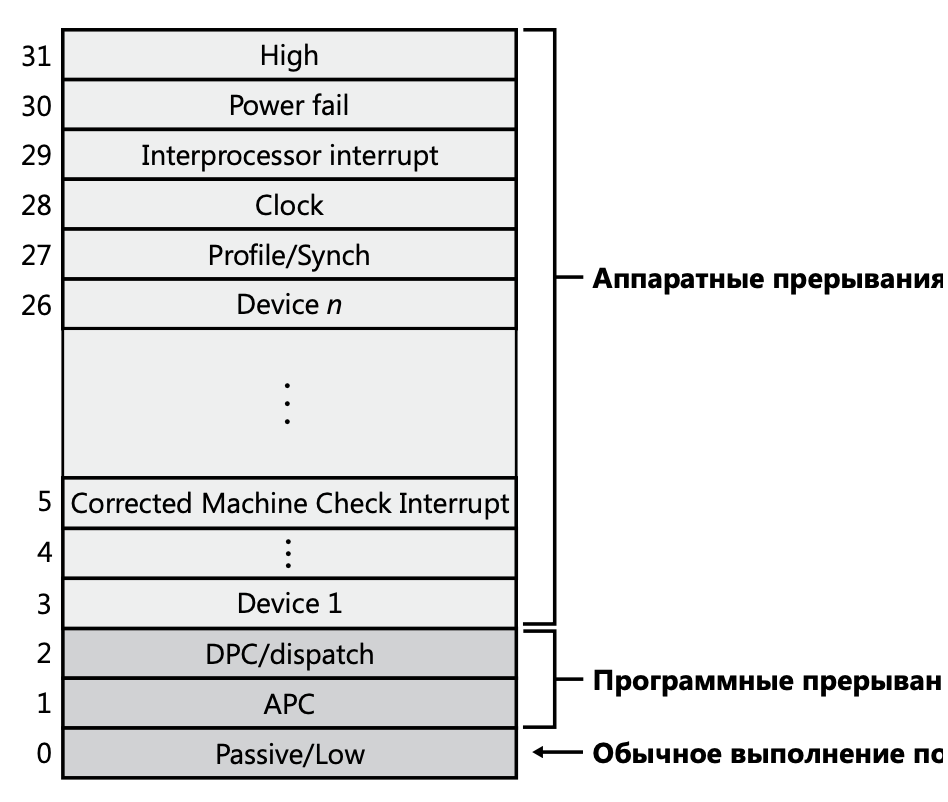
\includegraphics[width=150mm]{img/irql.png}
	\caption{Уровни  запросов прерываний (IRQL) для архитектуры x86}
	\label{fig:irql}
\end{figure}

ОС семейства Windows используют 32 уровня приоритета.
Приоритеты от 0 до 15 --- изменяющиеся уровни (из которых уровень 0 -- зарезервирован для потока обнуления страниц), а приоритеты от 16 до 31 --- приоритеты реального времени.


Уровни приоритета потоков назначаются исходя из двух разных позиций: одной от Windows API и другой от ядра Windows. Сначала Windows API систематизирует процессы по классу приоритета, который им присваивается при создании:
\begin{itemize}[label=---]
	\item Простоя --- Idle (1);
	\item Обычный --- Normal (2);
	\item Высокий --- High (3);
	\item Реального времени --- Real-time (4);
	\item Ниже обычного --- Below Normal (5);
	\item Выше обычного --- Above Normal (6).
\end{itemize}

После этого назначается относительный приоритет отдельных потоков внутри этих процессов:
\begin{itemize}[label=---]
	\item Простоя — Idle (–15);
	\item  Самый низший — Lowest (–2);
	\item Ниже обычного — Below-normal (–1);
	\item Обычный — Normal (0);
	\item Выше обычного — Above-normal (1);
	\item Наивысший — Highest (2);
	\item Критичный по времени — Time-critical (15).
\end{itemize}

Исходный базовый приоритет потока наследуется от базового приоритета процесса. Процесс по умолчанию наследует свой базовый приоритет у того процесса, который его создал. Соответствие между приоритетами Windows API и ядра системы приведено в таблице \ref{tbl:priority}


\begin{table}[h]
	\captionsetup{justification=raggedright,singlelinecheck=off,margin=2mm}
	\caption{Соответствие между приоритетами Windows API и ядра Windows}
	\begin{center}
		\begin{tabular}{|l|p{45pt}|p{45pt}|p{45pt}|p{45pt}|p{45pt}|p{45pt}|}
			\hline
			{} & \textbf{real-time} & \textbf{high} & \textbf{above normal} & \textbf{normal} & \textbf{below normal} & \textbf{idle}\\
			\hline
			\textbf{time critical} & 31 & 15 & 15 & 15 & 15 & 15 \\
			\hline
			\textbf{highest} & 26 & 15 & 12 & 10 & 8 & 6 \\
			\hline
			\textbf{above normal} & 25 & 14 & 11 & 9 & 7 & 5 \\
			\hline
			\textbf{normal} & 24 & 13 & 10 & 8 & 6 & 4 \\
			\hline
			\textbf{below normal} & 23 & 12 & 9 & 7 & 5 & 3 \\
			\hline
			\textbf{lowest} & 22 & 11 & 8 & 6 & 4 & 2 \\
			\hline
			\textbf{idle} & 16 & 1 & 1 & 1 & 1 & 1 \\
			\hline
		\end{tabular}
	\end{center}
	\label{tbl:priority}
\end{table}
\newpage

Текущий приоритет потока в динамическом диапазоне --- от 1 до 15 --- может быть повышен планировщиком вследствие причин, перечисленных ниже.

\begin{enumerate}[label={\arabic*.}]
	\item \textbf{Повышение приоритета вследствие событий планировщика или диспетчера (сокращение задержек)}
	
	При наступлении события диспетчера вызываются процедуры с целью проверки, не должны ли на локальном процессоре быть намечены какие-либо потоки, которые не должны быть спланированы. При каждом наступлении такого события вызывающий код может также указать, какого типа повышение должно быть применено к потоку, а также с каким приращением приоритета должно быть связано это повышение.
	
%	\item \textbf{Повышения приоритета, связанные с завершением ожидания}
%	
%	В общем случае поток, пробуждающийся из состояния ожидания, должен иметь возможность приступить к выполнению как можно скорее.
	
	%\item \textbf{Повышение приоритета владельца блокировки}
	
	\item \textbf{Повышение приоритета вследствии завершения ожидания}
	
	Такие повышения приоритета, пытаются уменьшить время задержки между потоком, пробуждающимся по сигналу объекта (переходя тем самым в состояние готовности), и потоком, фактически приступившим к своему выполнению в процессе, который не находился в состоянии ожидания (переходя тем самым в состояние выполнения). Поскольку событие, наступление которого ждал поток, может дать информацию того или иного сорта, скажем, о состоянии доступной на данный момент памяти, важно, чтобы это состояние не изменялось закулисно, пока поток все еще находится в состоянии готовности. В противном случае эта информация может стать неактуальной или неверной, как только поток будет запущен.
	
	\item \textbf{Повышение приоритета владельца блокировки}
	
	Поскольку блокировки ресурсов исполняющей системы и блокировки критических разделов используют основные объекты диспетчеризации, в результате освобождения этих блокировок осуществляются повышения приоритета, связанные с завершением ожидания.
	
	\item \textbf{Повышение приоритета вследствие завершения ввода-вывода }
	
	Windows дает временное повышение приоритета при завершении определенных операций ввода/вывода, при этом потоки, которые ожидали ввода/вывода имеют больше шансов сразу же запуститься. Подходящее значение для увеличения зависит от драйвера устройств (представлены в таблице \ref{tab:io}).

	
	\item \textbf{Повышение приоритета при ожидании ресурсов исполняющей системы}
	
	Если поток пытается получить ресурс исполняющей системы, который уже находится в исключительном владении другого потока, то он должен войти в состояние ожидания до тех пор, пока другой поток не освободит ресурс. Для ограничения риска взаимных исключений исполняющая система выполняет это ожидание, не входя в бесконечное ожидание ресурса, а интервалами по 5 секунд. Если по окончании этих 5 секунд ресурс все также находится во владении, то исполняющая система пытается предотвратить зависание центрального процессора путем получения блокировки диспетчера, повышения приоритета потока (потоков), владеющих ресурсом до 15 (в случае если исходный приоритет владельца был меньше, чем у ожидающего, и не был равен 15), перезапуска их квантов и выполнения еще одного ожидания.
	
	\clearpage
	
	\item \textbf{Повышение приоритета потоков первого плана после ожидания}
	
	Смысл такого повышения заключается в улучшении скорости отклика интерактивных приложений, то есть если дать приложениям первого плана небольшое повышение	приоритета при завершении ожидания, то у них повышаются шансы сразу же приступить к работе, особенно когда другие процессы с таким же базовым приоритетом	могут быть запущены в фоновом режиме.
	
	\item \textbf{Повышение приоритета после пробуждения GUI-потока}
	
	Потоки-владельцы окон получают при пробуждении дополнительное повышение приоритета на 2 из-за активности при работе с окнами, например, при поступлении сообщений от окна. Система работы с окнами ( Win32k.sys ) применяет это повышение приоритета, когда вызывает функцию KeSetEvent для установки события, используемого для пробуждения GUI-потока. Смысл такого повышения схож со смыслом 		предыдущего повышения — содействие интерактивным приложениям.
	
	\item \textbf{Повышения приоритета, связанные с перезагруженностью центрального процессора}
	
	Диспетчер настройки баланса (механизм ослабления загруженности центрального процессора) сканирует очередь готовых потоков раз в секунду и, если обнаружены потоки, ожидающие выполнения более 4 секунд, то диспетчер настройки баланса повышает их приоритет до 15. Как только квант истекает, приоритет потока снижается до базового приоритета. Если поток не был завершен за квант времени или был вытеснен потоком с более высоким приоритетом, то после снижения 		приоритета поток возвращается в очередь готовых потоков. Диспетчер настройки баланса сканирует лишь 16 готовых потоков и повышает приоритет не более чем у 10 потоков (если найдет) за один проход. При следующем проходе сканирование возобновляется	с того места, где оно было прервано в прошлый раз. 
	\clearpage
	
	
	\item \textbf{Повышение приоритетов для мультимедийных приложений и игр}
	
		Потоки, на которых выполняются различные мультимедийные приложения, должны выполняться с минимальными задержками. В Windows такая задача решается с помощью повышения приоритетов таких потоков драйвером \textbf{MMCSS (MultiMedia Class Scheduler Service)}. MMCSS работает с различными определенным задачи, например:
		\begin{enumerate}[label=\arabic*)]
			\item аудио;
			\item захват;
			\item распределение;
			\item игры;
			\item проигрывание;
			\item аудио профессионального качества
			\item задачи администратора многооконного режима.
		\end{enumerate}
\end{enumerate}

\begin{table}[h!]
	\caption{Рекомендуемые значения повышения приоритета.}
	\begin{center}
		\begin{tabular}{|p{100mm}|l|}
			\hline
			\textbf{Устройство} & \textbf{Приращение} \\
			\hline
			Диск, CD-ROM, параллельный порт, видео & 1 \\
			\hline
			Сеть, почтовый ящик, именованный канал, последовательный порт & 2 \\
			\hline
			Клавиатура, мышь & 6 \\
			\hline
			Звуковая плата & 8 \\
			\hline
		\end{tabular}
	\end{center}
	\label{tab:io}
\end{table}

Важное свойство для планирования потоков -- категория планирования -- это первичный фактор, который определяет приоритет потоков, зарегистрированных с MMCSS (категории планирования указаны в таблице \ref{tab:plan}).

Функции MMCSS временно повышают приоритет потоков, зарегистрированных с MMCSS до уровня, который соответствует категории планирования. Потом их приоритет снижается до уровня, соответствующего категории планирования Exhausted, для того, чтобы другие потоки тоже могли получить ресурс.
\begin{table}[h]
	\begin{center}
		\captionsetup{justification=raggedright,singlelinecheck=off,margin=2mm}
		\caption{Категории планирования.}
		\captionsetup{justification=raggedright,singlelinecheck=off,margin=2mm}
		\begin{tabular}{|p{40mm}|p{30mm}|p{80mm}|}
			\hline
			\textbf{Категория} & \textbf{Приоритет} & \textbf{Описание} \\
			\hline
			High (Высокая) & 23-26 & Потоки профессионального аудио (Pro Audio), запущенные с приоритетом выше, чем у других потоков на системе, за исключением критических системных потоков \\
			\hline
			Medium (Средняя) & 16-22 & Потоки, являющиеся частью приложений первого плана, например Windows Media Player \\
			\hline
			Low (Низкая) & 8-15 & Все остальные потоки, не являющиеся частью предыдущих категорий \\
			\hline
			Exhausted (Исчерпавших потоков) & 1-7 & Потоки, исчерпавшие свою долю времени центрального процессора, выполнение которых продолжиться, только если не будут готовы к выполнению другие потоки с более высоким уровнем приоритета \\
			\hline
		\end{tabular}
	\end{center}
	\label{tab:plan}
\end{table}
\section{UNIX}

Планирование процессов в UNIX основано на приоритете процесса. Планировщик всегда выбирает процесс с наивысшим приоритетом. Приоритеты планирования изменяются с течением времени (динамически) системой в зависимости от использования вычислительных ресурсов, времени ожидания запуска и текущего состояния процесса. 

Традиционное ядро UNIX является строго невытесняющим, однако в современных системах UNIX ядро является вытесняющим -- то есть процесс в режиме ядра может быть вытеснен более приоритетным процессом в режиме ядра. Ядро сделано вытесняющим для того, чтобы система могла обслуживать процессы реального времени, например видео и аудио.

Очередь процессов, готовых к выполнению, формируется согласно приоритетам и принципу вытесняющего циклического планирования, то есть сначала выполняются процессы с большим приоритетом, а процессы с одинаковым приоритетом выполняются в течении кванта времени друг за другом циклически. 
В случае, если процесс с более высоким приоритетом поступает в очередь процессов, готовых к выполнению, планировщик вытесняет текущий процесс и предоставляет ресурс более приоритетному процессу.

Приоритет процесса задается любым целым числом, которое лежит в диапазоне от 0 до 127 (чем меньше число, тем выше приоритет). Приоритеты 0 --- 49 зарезервированы для ядра (приоритеты ядра фиксированы), приоритеты 50 -- 127 являются прикладными  (приоритеты прикладных задач могут изменяться во времени)

Изменение приоритета прикладных задач зависит от степени <<любезности>> и от последней измеренной величины использования процессора.

Степень <<любезности>> --- это целое число в диапазоне от 0 до 39 со значением 20 по умолчанию. 
Увеличение значения приводит к уменьшению приоритета.
Пользователи могут повлиять на приоритет процесса при помощи изменения значений этого фактора, но только суперпользователь может увеличить приоритет процесса.
Фоновые процессы автоматически имеют более высокие значения этого фактора.

Структура proc содержит следующие поля, относящиеся к приоритетам:
\begin{enumerate}[label=\arabic*)]
	\item p\_pri --- текущий приоритет планирования;
	\item p\_usrpri --- приоритет режима задачи;
	\item p\_cpu --- результат последнего измерения использования процессора;
	\item p\_nice --- фактор <<любезности>>, который устанавливается пользователем.
\end{enumerate}

Значение \textbf{p\_pri} используется планировщиком для принятия решения о том, какой процесс направить на выполнение. Значения \textbf{p\_pri} и \textbf{p\_usrpri} равны, когда процесс находится в режиме задачи. 

Значение \textbf{p\_pri} может быть изменено (повышено) планировщиком для того, чтобы выполнить процесс в режиме ядра. В таком случае \textbf{p\_usrpri} будет использоваться для хранения приоритета, который будет назначен процессу, когда он вернется в режим задачи.

Поле \textbf{p\_cpu} инициализируется нулем при создании процесса, и на каждом тике обработчик таймера увеличивает это поле текущего процесса на 1, до максимального значения равного 127.

Ядро системы связывает приоритет сна с событием или ожидаемым ресурсом, из-за которого процесс может блокироваться (приоритет сна определяется для ярда, поэтому лежит в диапазоне 0 - 49). Когда процесс <<просыпается>>, ядро устанавливает \textbf{p\_pri}, равное приоритету сна события или ресурса, по которому произошла блокировка.
Значения приоритета сна для некоторых событий в системе 4.3BSD представлены в таблице \ref{tab:bsd}).

TODO: Здесь должна быть другая таблица из другой книги, не из Вахалии. Надо перебрать в tex, но мне лень, поэтому вот скрины: 

\begin{figure}[h]
	\centering
	\captionsetup{justification=centering}
	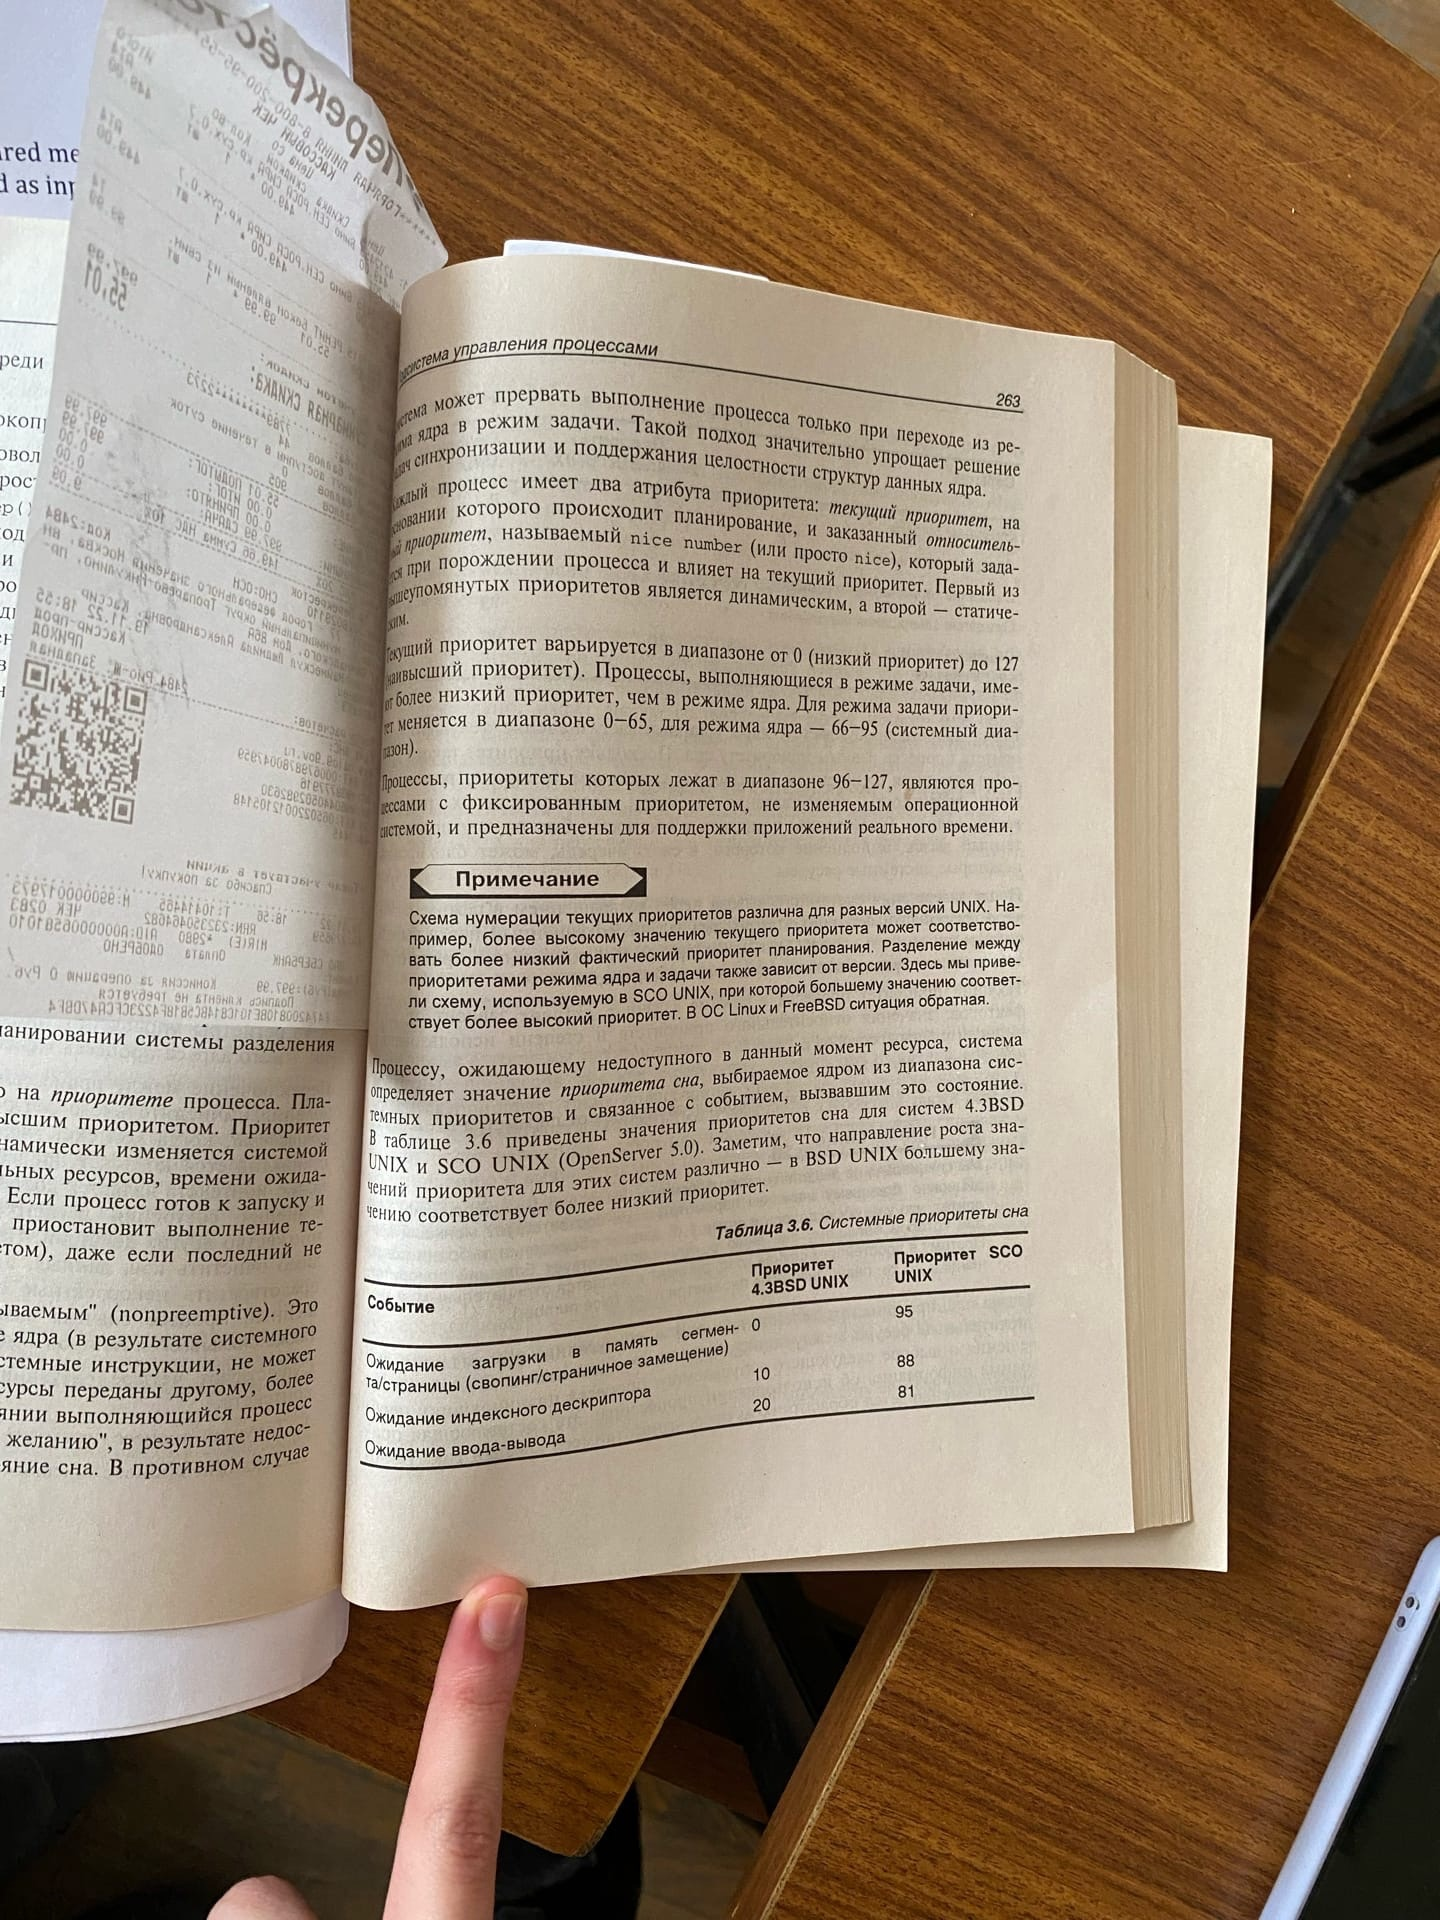
\includegraphics[width=150mm]{img/todo1.jpeg}
	\caption{TODO 1}
	\label{fig:todo1}
\end{figure}

\begin{figure}[h]
	\centering
	\captionsetup{justification=centering}
	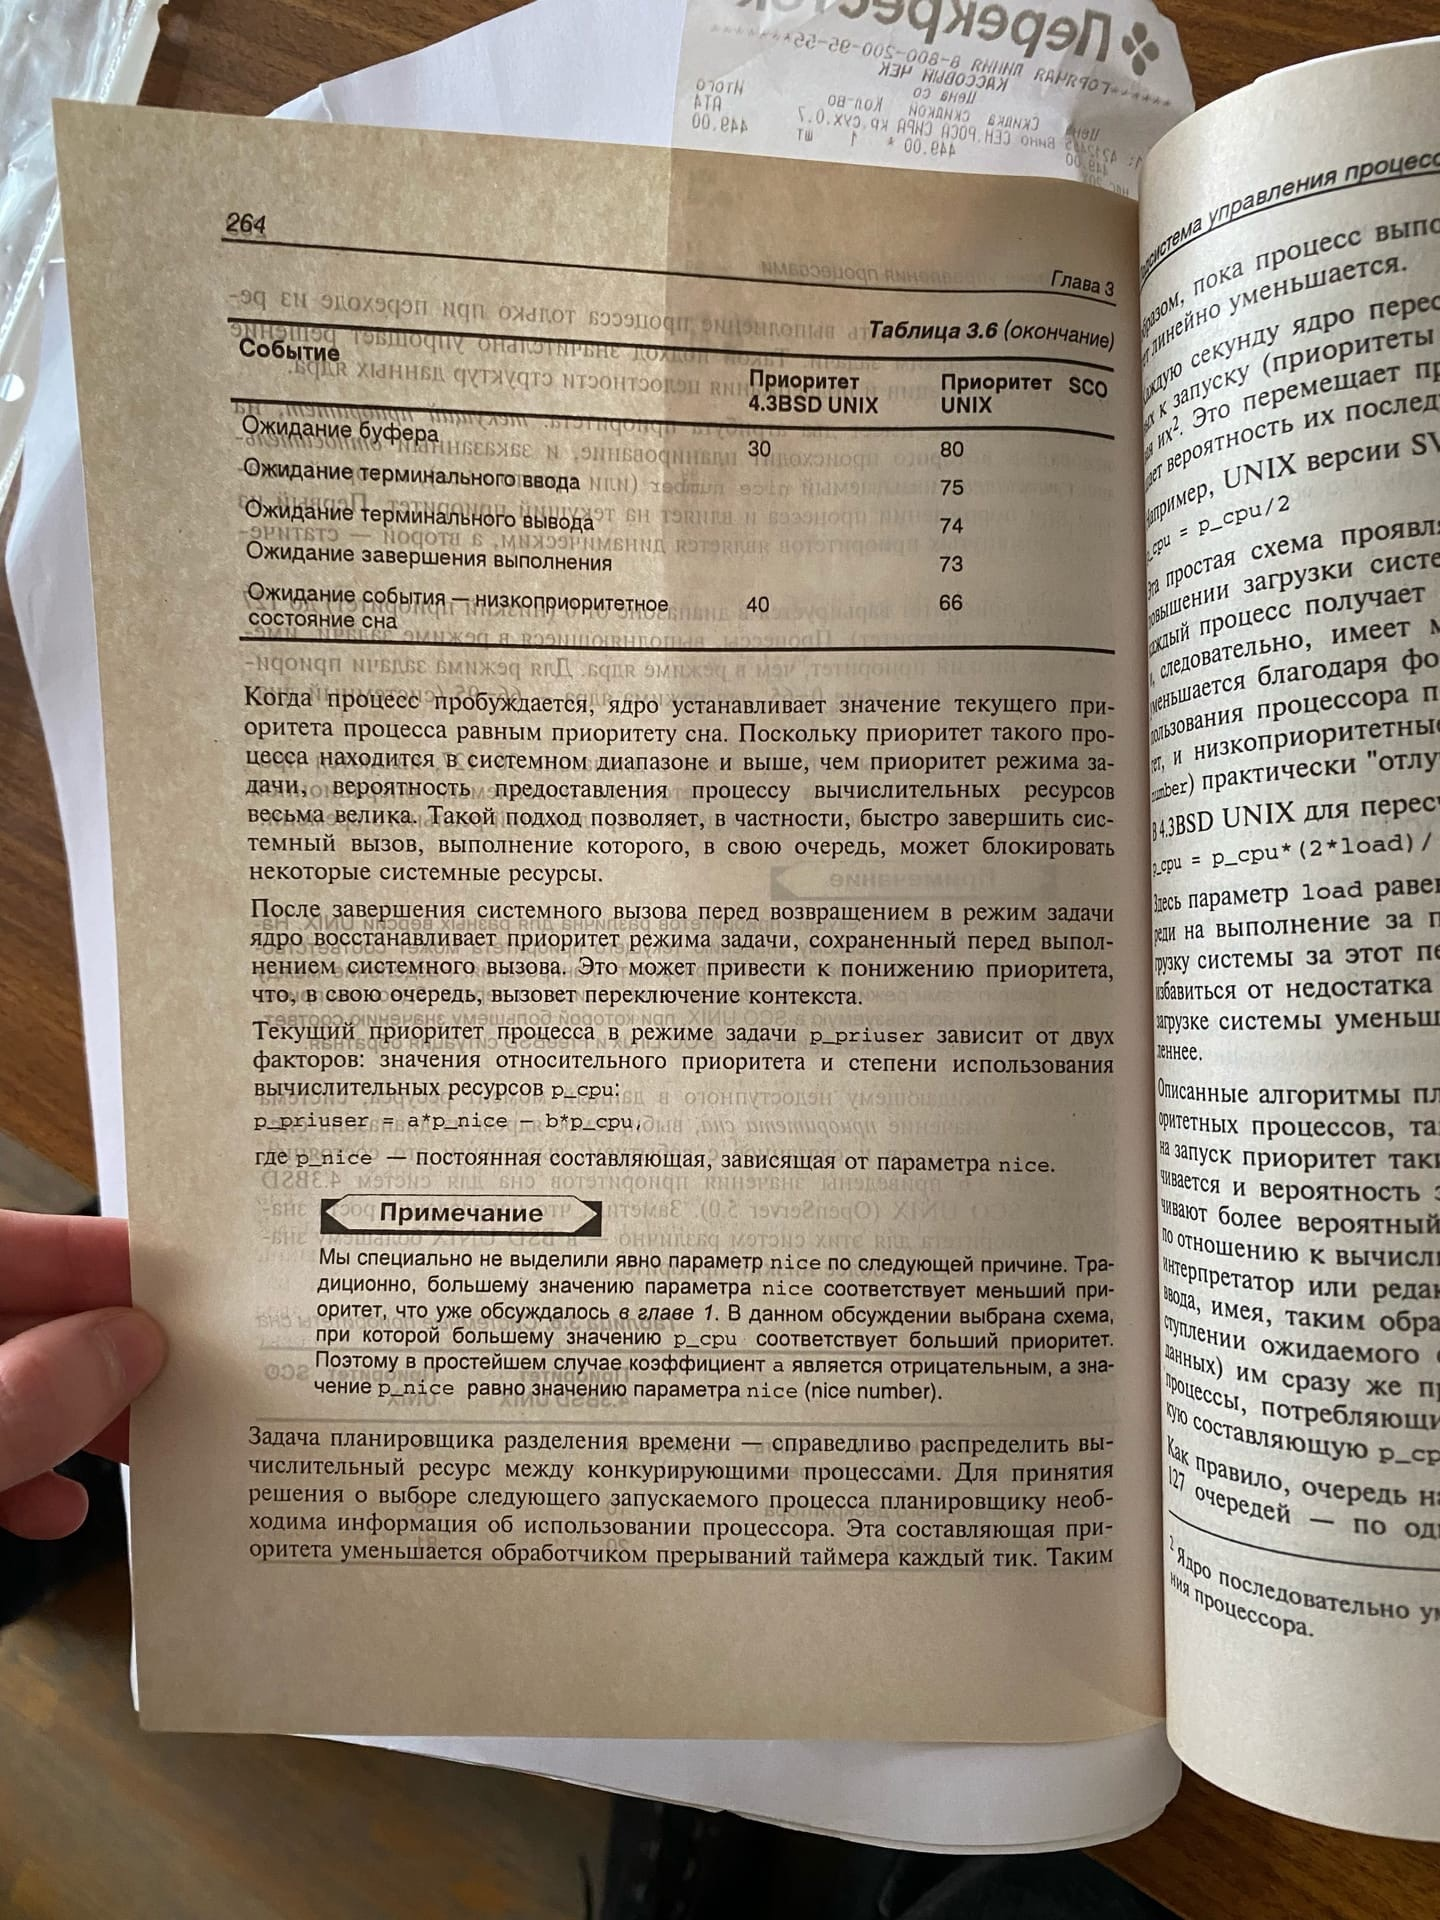
\includegraphics[width=150mm]{img/todo2.jpeg}
	\caption{TODO 2}
	\label{fig:todo2}
\end{figure}

\begin{table}[h]
	\captionsetup{justification=raggedright,singlelinecheck=off,margin=2mm}
	\caption{Приоритеты
		сна в ОС \textbf{4.3BSD}}
	\label{tab:bsd}
	\begin{center}
		\begin{tabular}{ |c|c|c|  }
			\hline
			\textbf{Приоритет} & \textbf{Значение} & \textbf{Описание} \\
			\hline
			\texttt{PSWP} & 0 & Свопинг \\
			\hline
			\texttt{PSWP + 1} & 1 & Страничный демон \\
			\hline	
			\texttt{PSWP + 1/2/4} & 1/2/4 & Другие действия по обработке памяти \\
			\hline
			\texttt{PINOD} & 10 & Ожидание освобождения inode \\
			\hline
			\texttt{PRIBIO} & 20 & Ожидание дискового ввода-вывода \\
			\hline
			\texttt{PRIBIO + 1} & 21 & Ожидание освобождения буфера \\
			\hline
			\texttt{PZERO} & 25 & Базовый приоритет \\
			\hline
			\texttt{TTIPRI} & 28 & Ожидание ввода с терминала \\
			\hline
			\texttt{TTOPRI} & 29 & Ожидание вывода с терминала \\
			\hline 
			\texttt{PWAIT} & 30 & Ожидание завершения процесса потомка \\
			\hline
			\texttt{PLOCK} & 35 & Консультативное ожидание блок. ресурса \\
			\hline
			\texttt{PSLEP} & 40 & Ожидание сигнала \\
			\hline
		\end{tabular}
	\end{center}
\end{table}

Каждую секунду ядро системы инициализирует отложенный вызов процедуры schedcpu(), которая уменьшает значение \textbf{p\_pri} каждого процесса исходя из фактора <<полураспада>> (в системе 4.3BSD считается по формуле \ref{eq:ref1}).
\begin{equation}
	\label{eq:ref1}
	decay = \frac{2 \cdot load\_average}{2 \cdot load\_average + 1},
\end{equation} где
\textit{load\_average} - это среднее количество процессов, находящихся в состоянии готовности к выполнению, за последнюю секунду.

Также процедура schedcpu() пересчитывает приоритеты для режима задачи
всех процессов по формуле \ref{eq:ref2}.
\begin{equation}
	\label{eq:ref2}
	p\_usrpri = PUSER + \frac{p\_cpu}{2} + 2 \cdot p\_nice,
\end{equation}где \textit{PUSER} - базовый приоритет в режиме задачи, равный 50.

Таким образом, если процесс в последний раз использовал большое количество процессорного времени, то его р\_срu будет увеличен => рост значения p\_usrpri => понижение приоритета.  Чем дольше процесс простаивает в очереди на выполнение, тем больше фактор полураспада уменьшает его р\_срu => повышение его приоритета. Такая схема предотвращает бесконечное откладывание низкоприоритетных процессов. Применение данной схемы предпочтительно процессам, осуществляющим много операций ввода-вывода, в противоположность процессам, производящим много вычислений. То есть динамический пересчет приоритетов процессов в режиме задачи позволяет избежать бесконечного откладывания.


\chapter{Вывод}
Функции обработчика прерывания от системного таймера в системах разделения времени семейства UNIX и для семейства Windows схожи, так как эти ОС являются системами разделения времени с динамическими приоритетами и вытеснением.. Общие основные функции:
\begin{enumerate}[label=\arabic*)]
	\item декремент кванта текущего процесса в UNIX и декремент текущего потока в Windows;
	\item инициализация отложенных действий, которые относятся к работе планировщика (например пересчет приоритетов);
	\item декремент счетчиков времени (таймеров, часов, счетчиков времени отложенных действий, будильников реального времени).
\end{enumerate}


Пересчёт динамических приоритетов осуществляется только для пользовательских процессов для того, чтобы избежать бесконечного откладывания.

\clearpage


\begin{table}[h]
	\captionsetup{justification=raggedright,singlelinecheck=off,margin=2mm}
	\caption{Приоритеты
		сна в ОС \textbf{4.3BSD}}
	\label{tab:bsd}
	\begin{center}
		\begin{tabular}{ |c|c|c|  }
			\hline
			\textbf{Приоритет} & \textbf{Значение} & \textbf{Описание} \\
			\hline
			\texttt{PSWP} & 0 & Свопинг \\
			\hline
			\texttt{PSWP + 1} & 1 & Страничный демон \\
			\hline	
			\texttt{PSWP + 1/2/4} & 1/2/4 & Другие действия по обработке памяти \\
			\hline
			\texttt{PINOD} & 10 & Ожидание освобождения inode \\
			\hline
			\texttt{PRIBIO} & 20 & Ожидание дискового ввода-вывода \\
			\hline
			\texttt{PRIBIO + 1} & 21 & Ожидание освобождения буфера \\
			\hline
			\texttt{PZERO} & 25 & Базовый приоритет \\
			\hline
			\texttt{TTIPRI} & 28 & Ожидание ввода с терминала \\
			\hline
			\texttt{TTOPRI} & 29 & Ожидание вывода с терминала \\
			\hline 
			\texttt{PWAIT} & 30 & Ожидание завершения процесса потомка \\
			\hline
			\texttt{PLOCK} & 35 & Консультативное ожидание блок. ресурса \\
			\hline
			\texttt{PSLEP} & 40 & Ожидание сигнала \\
			\hline
		\end{tabular}
	\end{center}
\end{table}







